\documentclass[french]{pfia}

% ------------------------------------------
% TITRE
% ------------------------------------------

\title{\textbf{
%Un langage dédié pour le calcul par contraintes d'emplois du temps universitaires
A domain-specific language for university timetabling
}}
\usepackage{tabularx}
\usepackage{mathtools}
\usepackage{url}
\usepackage{stmaryrd}%for denotational brackets
\usepackage{nccmath}
\usepackage{todonotes}
% please place your own definitions here and don't use \def but
% \newcommand{}{}

%%%%%%%%%%%%%%%%%%%%%%%%%%%%%%%%%%%%%%%%%%%%%%%%%%%%
%% ACRONYMS
\newcommand{\acronym}[1]{{\texttt{#1}}}

\newcommand{\CHR}{\acronym{CHR}}
\newcommand{\C}{\acronym{C}}
\newcommand{\CPP}{\acronym{C++}}
\newcommand{\CSS}{\acronym{CSS}}
\newcommand{\DZN}{\acronym{DZN}}
\newcommand{\FLATZINC}{\acronym{Flatzinc}}
\newcommand{\GECODE}{\acronym{Gecode}}
\newcommand{\JSON}{\acronym{JSON}}
\newcommand{\JAVA}{\acronym{Java}}
\newcommand{\LISP}{\acronym{Lisp}}
\newcommand{\MINIZINC}{\acronym{MiniZinc}}
\newcommand{\PROLOG}{\acronym{Prolog}}
\newcommand{\XML}{\acronym{XML}}
\newcommand{\CHRPP}{\acronym{CHR++}}

\newcommand{\CP}{\acronym{CP}}
\newcommand{\CSP}{\acronym{CSP}}
\newcommand{\DSL}{\acronym{DSL}}
\newcommand{\ITC}{\acronym{ITC}}
\newcommand{\NP}{\acronym{NP}}
\newcommand{\SAT}{\acronym{SAT}}
\newcommand{\UTP}{\acronym{UTP}}


%%%%%%%%%%%%%%%%%%%%%%%%%%%%%%%%%%%%%%%%%%%%%%%%%%%%
%% UTP BUILT-IN TYPES
\newcommand{\SLOT}{H}

\newcommand{\COURSES}{C^{*}}
\newcommand{\COURSE}{C}
\newcommand{\PART}{P}
\newcommand{\CLASS}{K}
\newcommand{\SESSION}{S}

\newcommand{\STUDENT}{U}
\newcommand{\GROUP}{G}
\newcommand{\TEACHER}{T}
\newcommand{\ROOM}{R}

%%%%%%%%%%%%%%%%%%%%%%%%%%%%%%%%%%%%%%%%%%%%%%%%%%%%
%% UTP TYPES
\newcommand{\TYPE}{\mathcal{E}}
\newcommand{\ENTITY}{E}
\newcommand{\EMAP}{F}

\newcommand{\LABEL}{\mathcal{L}}
\newcommand{\RANK}{\mathcal{O}}
\newcommand{\SELECTOR}{\mathcal{F}}

%%%%%%%%%%%%%%%%%%%%%%%%%%%%%%%%%%%%%%%%%%%%%%%%%%%%
%% UTP PROPERTIES
\newcommand{\proptype}[2]{#1^{#2}}
\newcommand{\prop}[3]{\proptype{#1}{#2}_{#3}}

\newcommand{\WEEK}{w}
\newcommand{\WEEKDAY}{d}
\newcommand{\DAILYSLOT}{m}

\newcommand{\PARTALLOWEDSLOT}{d}
\newcommand{\SESSIONDURATION}{length}
\newcommand{\SESSIONRANK}{rank}
\newcommand{\CLASSCAPACITY}{maxsize}
\newcommand{\ROOMCAPACITY}{capacity}
\newcommand{\ROOMDISJUNCTIVE}{disjunct}
\newcommand{\PARTROOMDEMAND}{multi}
\newcommand{\PARTTEACHERDEMAND}{team}
\newcommand{\PARTTEACHERSESSIONS}{service}
\newcommand{\CLASSPARENT}{parents}

\newcommand{\partallowedslots}[1]{\prop{\PARTALLOWEDSLOT}{\SESSION,\SLOT}{#1}}
\newcommand{\sessionduration}[1]{\prop{\SESSIONDURATION}{\SESSION}{#1}}
\newcommand{\rankedsessions}{O}
%\newcommand{\sessionrank}[1]{\prop{\SESSIONRANK}{\SESSION}{#1}}
\newcommand{\classcapacity}[1]{\prop{\CLASSCAPACITY}{\CLASS}{#1}}
\newcommand{\roomcapacity}[1]{\prop{\ROOMCAPACITY}{\ROOM}{#1}}
%\newcommand{\roomdisjunctive}[1]{\prop{\ROOMDISJUNCTIVE}{\ROOM}{#1}}
\newcommand{\disjunctiverooms}{D}%{\ROOMDISJUNCTIVE}
%\newcommand{\oneroom}[1]{\prop{\PARTROOMDEMAND}{\PART}{#1}}
\newcommand{\multiroomparts}{M}%{\PARTROOMDEMAND}
\newcommand{\partteachermultiplicity}[1]{\prop{\PARTTEACHERDEMAND}{\PART}{#1}}
\newcommand{\partteacherservice}[1]{\prop{\PARTTEACHERSESSIONS}{{\TEACHER}\times{\PART}}{#1}}
\newcommand{\classparent}[1]{\prop{\CLASSPARENT}{\CLASS,\CLASS}{#1}}


%%%%%%%%%%%%%%%%%%%%%%%%%%%%%%%%%%%%%%%%%%%%%%%%%%%%
%% UTP MAPS
\newcommand{\maptype}[2]{d^{#1,#2}}
\newcommand{\map}[3]{\maptype{#1}{#2}_{#3}}

%%%%%%%%%%%%%%%%%%%%%%%%%%%%%%%%%%%%%%%%%%%%%%%%%%%%
%% UTP PREDICATES

%{\ADJACENTROOMS}
%{\ATMOSTDAILY}
%{\ATMOSTWEEKLY}
%{\TRAVEL}
%{\FORBIDDENPERIOD}
%{\NOOVERLAP}
%{\SAMEDAILYSLOT}
%{\SAMEDAY}
%{\SAMEROOMS}
%{\SAMESLOT}
%{\SAMESTUDENTS}
%{\SAMETEACHERS}
%{\SAMEWEEKDAY}
%{\SAMEWEEKLYSLOT}
%{\SAMEWEEK}
%{\SEQUENCED}
%{\TEACHERDISTRIBUTION}
%{\WEEKLY}

\newcommand{\ADJACENTROOMS}{adjacent\_rooms}
\newcommand{\ATMOSTDAILY}{at\_most\_daily}
\newcommand{\ATMOSTWEEKLY}{at\_most\_weekly}
\newcommand{\TRAVEL}{travel}
\newcommand{\FORBIDDENPERIOD}{forbidden\_period}
\newcommand{\NOOVERLAP}{no\_overlap}
\newcommand{\SAMEDAILYSLOT}{same\_daily\_slot}
\newcommand{\SAMEDAY}{same\_day}
\newcommand{\SAMEROOMS}{same\_rooms}
\newcommand{\SAMESLOT}{same\_slot}
\newcommand{\SAMESTUDENTS}{same\_students}
\newcommand{\SAMETEACHERS}{same\_teachers}
\newcommand{\SAMEWEEKDAY}{same\_weekday}
\newcommand{\SAMEWEEKLYSLOT}{same\_weekly\_slot}
\newcommand{\SAMEWEEK}{same\_week}
\newcommand{\SEQUENCED}{sequenced}
\newcommand{\TEACHERDISTRIBUTION}{teacher\_distribution}
\newcommand{\WEEKLY}{weekly}
%\newcommand{\NOOVERLAP}{no-overlap}

%allocation\_group
%assign
%domain\_class\_group
%domain\_class\_room
%domain\_session\_teacher
%part\_schedule



%%%%%%%%%%%%%%%%%%%%%%%%%%%%%%%%%%%%%%%%%%%%%%%%%%%%
%% CP VARIABLES
\newcommand{\vartype}[2]{x^{#1,#2}}
\newcommand{\var}[3]{\vartype{#1}{#2}_{#3}}

%% AUXILIARY VARIABLES
\newcommand{\CLASSSIZE}{size}
\newcommand{\ROOMUSE}{use}
%\newcommand{\SESSIONEND}{end}

\newcommand{\classsize}[1]{\prop{\CLASSSIZE}{}{}(#1)}%{\CLASS}{#1}}
\newcommand{\roomuse}[4]{y_{#1,#2,#3,#4}}
%\newcommand{\roomuse}[4]{\prop{\ROOMUSE}{}{}(#1,#2,#3,#4)}
%\newcommand{\sessionend}[1]{\prop{\SESSIONEND}{}{}(#1)}%{\SESSION,\SLOT}{#1}}

%% AUXILIARY VARIABLES REIFYING CONSTRAINTS
\newcommand{\DISJOINT}{split}
\newcommand{\disjoint}[2]{\prop{\DISJOINT}{}{}(#1,#2)}%{\SESSION\times\SESSION}{#1#2}}
\newcommand{\disjointroom}[3]{\prop{\DISJOINT}{}{}(#1,#2,#3)}%{\SESSION\times\SESSION}{#1#2}}


%%%%%%%%%%%%%%%%%%%%%%%%%%%%%%%%%%%%%%%%%%%%%%%%%%%%
%% Maths
\newcommand{\BOOLEAN}{\mathbb{B}}
\newcommand{\NATURAL}{\mathbb{N}}
\newcommand{\myset}[1]{\{#1\}}
\newcommand{\mycard}[1]{|#1|}
\newcommand{\setunion}[3]{\cup_{#1 \in #2}#3}
\newcommand{\setintersection}[3]{\cap_{#1 \in #2}#3}
\newcommand{\setpartition}[3]{\sqcup_{#1 \in #2}#3}
\newcommand{\denote}[1]{\llbracket #1\rrbracket}

%%%%%%%%%%%%%%%%%%%%%%%%%%%%%%%%%%%%%%%%%%%%%%%%%%%%
%% Minizinc syntaxe

% \newcommand{\forallmzn}{\text{forall }}
% \newcommand{\arrowmzn}{\text{->}}
% \newcommand{\inmzn}{\text{ in }}
% \newcommand{\wmzn}{\text{ where }}
% \newcommand{\arraymzn}[1]{\text{#1}}
% \newcommand{\funcmzn}[1]{\text{#1}}
% \newcommand{\gconst}[1]{\text{#1}}
% \newcommand{\const}{\text{constraint  }}
% \newcommand{\subsetmzn}{\text{ subset }}
% \newcommand{\summzn}{\text{sum }}
% \newcommand{\divmzn}{\text{ div }}
% \newcommand{\modmzn}{\text{mod }}
% \newcommand{\intermzn}{\text{ intersect }}
% \newcommand{\equimzn}{\text{<=>}}
% \newcommand{\leqmzn}{\text{>=}}
% \newcommand{\geqmzn}{\text{<=}}

%% Minizinc
\newcommand{\forallmzn}{\text{forall}}
\newcommand{\arrowmzn}{\texttt{ -> }}
\newcommand{\inmzn}{\text{ in }}
\newcommand{\wmzn}{\text{ where }}
\newcommand{\arraymzn}[1]{\text{#1}}
\newcommand{\funcmzn}[1]{\text{#1}}
\newcommand{\gconst}[1]{\text{#1}}
\newcommand{\const}{\text{constraint  }}
\newcommand{\subsetmzn}{\text{ subset }}
\newcommand{\summzn}{\text{sum}}
\newcommand{\divmzn}{\text{ div }}
\newcommand{\modmzn}{\text{ mod }}
\newcommand{\intermzn}{\text{ intersect }}
\newcommand{\equimzn}{\text{<=>}}
\newcommand{\leqmzn}{\texttt{>=}}
\newcommand{\gqmzn}{\texttt{<}}
\newcommand{\lqmzn}{\texttt{>}}
\newcommand{\geqmzn}{\texttt{<=}}
\newcommand{\neqmzn}{\texttt{!=}}
\newcommand{\landmzn}{\text{ /\textbackslash \, }}
\newcommand{\lormzn}{\text{ \textbackslash /}}
\newcommand{\existmzn}{\text{exists}}
\newcommand{\notmzn}{\text{not}}


%% Minizinc 


\newcommand{\xgroup}{\text{x\_groups}}
\newcommand{\xstudent}{\text{x\_group}}
\newcommand{\xroom}{\text{x\_rooms}}
\newcommand{\xteacher}{\text{x\_lecturers}}
\newcommand{\xslot}{\text{x\_slot}}

%% CHR syntax
\newcommand{\xslotstart}{\text{x\_slot\_start}}
\newcommand{\xslotend}{\text{x\_slot\_end}}
\newcommand{\arraychr}[1]{\text{#1}}
\newcommand{\funcchr}[1]{\text{#1}}
\newcommand{\ctchr}[1]{\texttt{#1}}
\newcommand{\chrprop}{\Rightarrow}
\newcommand{\chrsimpl}{\Leftrightarrow}

\newcommand{\davidg}[1]{\todo[inline,color=orange!40]{#1}}
\newcommand{\davidl}[1]{\todo[inline,color=yellow!40]{#1}}
\newcommand{\vincent}[1]{\todo[inline,color=blue!40]{#1}}
\newcommand{\marc}[1]{\todo[inline,color=green!40]{#1}}
\newcommand{\corentin}[1]{\todo[inline,color=pink]{#1}}

% ------------------------------------------
% AUTEUR(S)
% ------------------------------------------

% 1 auteur
% \author{L. Auteur \\
%  Organisme de rattachement, acronyme laboratoire}
% \date{mél}
 
% plusieurs auteurs 
\author{Vincent Barichard, Corentin Behuet, David Genest, Marc Legeay, David Lesaint\\[6pt]
%\fup{1} Organisme de rattachement 1, acronyme laboratoire 1\\
Univ Angers, LERIA, F-49000 Angers, France \\
%\fup{2} Organisme de rattachement 2, acronyme laboratoire 2\\
%\fup{3} Organisme de rattachement 3, acronyme laboratoire 3\\
}

\date{
\{prenom.nom\}@univ-angers.fr
}

\begin{document}

\maketitle

% ------------------------------------------
% RÉSUMÉS ET MOTS-CLÉS
% ------------------------------------------

\begin{resume}
%Le calcul d'emplois du temps universitaires est un problème d'optimisation combinatoire complexe tant dans sa modélisation que sa résolution. Peu de travaux se sont intéressés dans l'état de l'art aux particularités du système universitaire français et nous présentons dans ce cadre une approche par contraintes pour le calcul d'emplois du temps. Cette approche se fonde sur un langage dédié à base de règles, le schéma {\UTP}, permettant de modéliser les différentes entités et contraintes d'une instance. La résolution repose quant à elle sur un modèle générique développé en {\MINIZINC} ainsi qu'un parser qui permet de compiler toute instance {\UTP} dans un langage de programation par contraintes et de la résoudre par un solver de contraintes. Nous présentons quelques expérimentations préliminaires menées sur des instances réelles.

La planification des cours universitaires est un problème d'optimisation combinatoire complexe, tant dans sa modélisation que dans sa résolution.
Il recouvre plusieurs problèmes~: la répartition des étudiants, la planification des salles et des services d'enseignements, l'ordonnancement des cours et l'allocation des ressources.
Dans cet article, nous présentons un langage dédié à base de règles, le langage \UTP{}, qui permet de modéliser les différentes entités et contraintes du problème.
Nous comparons le langage \UTP{} à d'autres approches de résolution pour la construction d'emploi du temps.
Comme preuve de concept, nous avons implémenté des modèles en programmation par contraintes et les avons expérimentés sur des instances réelles provenant d'une université française.
\end{resume}

\begin{motscles}
Emploi du temps universitaire $\bullet$ Langage dédié $\bullet$ Programmation par contraintes 
\end{motscles}

%\begin{abstract}
%The computation of university timetables is a complex combinatorial optimisation problem both in its modelling and its solution. Few works in the state of the art have focused on the particularities of the French university system and we present in this context a constraint-based approach for the computation of timetables. This approach is based on a dedicated rule-based language, the {\UTP} scheme, which allows to model the different entities and constraints of an instance. The resolution is based on a generic model developed in {\MINIZINC} as well as a parser that allows to compile any instance {\UTP} in a constraint programming language and to solve it by a constraint solver. We present some preliminary experiments conducted on real instances.
%\end{abstract}

% JFPC:
%Le calcul d'emplois du temps universitaire est un problème d'optimisation combinatoire complexe tant dans sa modélisation que sa résolution.
%Nous présentons une approche par contraintes qui englobe la constitution de groupes, la distribution des salles et enseignants, leur allocation et l'ordonnancement des séances.
%Cette approche se fonde sur un langage dédié à base de règles ({\UTP}) permettant de modéliser les différentes entités et contraintes d'une instance.
%Les instances \UTP{} sont encodées en \XML{} et un parseur convertit les règles en contraintes dans un format \JSON{} compatible avec les solveurs \MINIZINC{} et \CHR{}.
%Nous présentons ici le modèle \MINIZINC{} pour la classe \UTP{} et des expérimentations préliminaires réalisées sur des instances réelles issues du système universitaire francais.

\begin{abstract}
University course timetabling is a complex combinatorial optimisation problem both in its modeling and its solving.
It involves several problems\string: student sectioning, course staffing, room planning, class scheduling and resource allocation.
In this paper we present a dedicated rule-based language, the \UTP{} language, which allows to model the different entities and constraints of the problem.
We compare the \UTP{} language with other timetabling frameworks.
As a proof of concept, we developed constraint programming solvers and performed experiments on real instances from a French university.
\end{abstract}

\begin{keywords}
University Timetabling $\bullet$ Domain-Specific Language $\bullet$ Constraint Programming
\end{keywords}

% ------------------------------------------
% CORPS DE L'ARTICLE
% ------------------------------------------

%------------------------------------------------------------
%------------------------------------------------------------
\section{Introduction}
\label{sec:introduction}

Course organization %in universities
involves strategic, tactical and operational decisions relating to curriculum design, student sectioning, course staffing, room planning, 
%equipment provisioning, 
class scheduling and resource allocation \cite{overview_uctp_2016_malaysian}.
The scope %and dynamics 
of these problems and the coordination of the different stages
vary between higher-education systems and institutions 
as does the level of process automation and decision tool support.
In french universities for instance, curricula are conventionally revisited every 5 years and 
students enroll in courses prior to each teaching period in the course of the academic year. %and are partitioned into groups based on their demand profile. 
Demand is matched by sectioning courses into classes, partitioning students %with identical profiles 
into fixed groups, and populating classes with groups. %to match demand.
Eligible groups, %faculty 
teachers, rooms and equipment are then identified for each course before class sessions get scheduled and allocated the necessary resources (see Figure~\ref{fig:utp-workflow}). 
Each stage involves 
different stakeholders with their own requirements
(faculty departments, administrative units, course owners, lecturers, etc.) 
and the workflow naturally allows for deviations and contingencies (marginal amendments to curricula on a yearly basis, late student registrations, staff absences, etc.).

% For one-column wide figures use
\begin{figure}[h]
\begin{center}
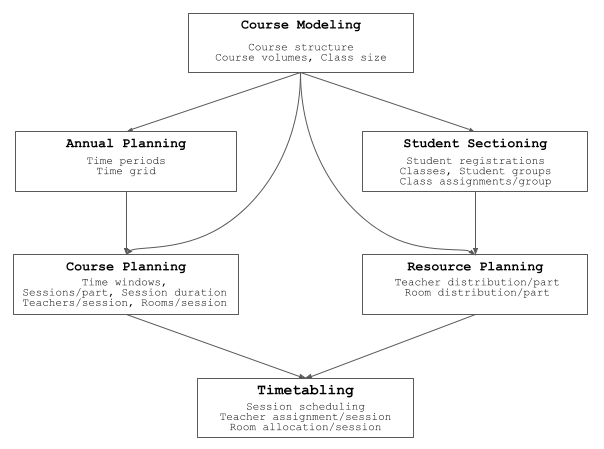
\includegraphics[width=\columnwidth]{img/utp_workflow.png}
\end{center}
\caption{Conventional workflow for course organization in french universities}%: steps and roles}

\label{fig:utp-workflow}
\end{figure}

We introduce in this paper a domain-specific language modeling a broad class of university timetabling problems ({\UTP}) that reduce to hard constraint satisfaction problems ({\CSP}). 
The {\UTP} language allows to mix and match features relating to course scheduling, resource allocation and student sectioning in order to tailor problem instances to each particular environment.
It is designed around a formal domain model and a predicate language to state rules and constraints. 
Each instance is decomposed into a model of entities and maps, a rule set and a solution component. 
Rules express collections of timetabling constraints %that represent 
%assignment decisions %, domain restrictions 
%and general 
%timetabling constraints 
on model entities and 
the solution component %is a list of choices made for some or all of the decisions at stake % (e.g., start time of a session) 
lists assignment decisions. 
The latter does not have to be exhaustive (e.g., it may be void), nor consistent. 
{\UTP} instances may therefore be used to model subproblems and solution seeds %when the whole problem is solved in successive stages (e.g., sequential workflows chaining student sectioning, course scheduling and resource allocation). 
%Since no assumption is made on the computing task, 
%{\UTP} instances may also be used
either to repair timetables, complete partial timetables or generate full solutions. 

%Similarly to the schema proposed in \cite{2018muller,ITC2019} for the international timetabling competition ({\ITC}), 
The {\UTP} model adopts:
\begin{itemize}
    \item a multi-scale schedule horizon, i.e., weeks, weekdays and daily slots ;
    \item a mixed set of resources, i.e., students, rooms and teachers ;
    \item a hierarchical course structure, i.e., a course (e.g. algorithmic) contains course parts (e.g., algorithmic practice), a course part contains classes (e.g., algorithmic practice for student group G1a), and a class contains sessions (e.g., the third session of algorithmic practice for G1a).
\end{itemize}
In our approach, class sessions are considered as first-class objects that must be scheduled individually alongside resources. %For full flexibility, 
%\todo[inline]{"part classes" on n'utilise plus ce terme après, mais "class", donc je trouve que c'est piégeux, parce que ce dont on parle ici "part classes" est appelé plus tard "class". Je sais que l'intro est déjà longue, mais je m'interroge quand même sur l'intérêt de ne pas donner plus de détails (à la place de "i.e. course parts...") du type "i.e. a course (e.g. algorithmic) contains course parts (e.g. algorithmic lectures), a course part contains classes (e.g. algorithmic lectures for student group G1a), and a class contains sessions (e.g. the third session of algorithmic lecture for G1a)". C'est à mon avis très important que lecteur comprenne les termes dès le début de l'intro. }
%\marc{On n'utilise jamais "course parts", "part classes" et "class sessions" mais "part", "classes" et "sessions", ici je ne trouve pas ça gênant d'insister sur le lien puisqu'on parle de la hiérarchie ?}
%\todo[inline]{DL : Il faut savoir que ce n'est pas le cas dans ITC, est-ce que le lecteur "visé" le sait ? Ca ne vaudrait pas le coup d'en dire un mot ?}
%\marc{En relisant c'est bien indiqué "in our approach however" donc ça indique bien que ce n'est pas le cas pour ITC ?}
The scheduling scheme assumes cumulative resources and multi-resource sessions 
but may be adapted to each instance using entity properties and maps. 
Specifically, 
sessions are cast as single-resource %tasks 
(e.g., face-to-face lectures) or multi-resource tasks (e.g., hybrid sessions) %using multiplicity marking 
by quantifying the needed resources. 
%In either case, 
Candidate resources for a session are identified based on the distribution that is given over courses (i.e., registered students) and course parts (i.e., designated teachers and rooms). 
The volumes of sessions are themselves configurable for teachers (i.e., sessions quota per course part) but pre-determined for students (i.e., mandatory session attendance per class) while rooms may be reused at will. %within course part boundaries. 

No limits apply on simultaneous resource usage but for rooms whose hosting capacity must match %cumulated 
class size. 
As for session scheduling, start time grids are configurable in each course part and 
the model simply requires full session sequencing in each class. 
Any resource may therefore be assigned simultaneous or overlapping sessions  (e.g., joint sessions, optional tutoring) except for rooms assigned to a multi-room session. 
Note that disjunctive rules may be enforced as needed to prevent parallelism or impose unit resources. 
%are subject to class-scoped global sequencing constraints 
%
%Lastly, the model sections students into classes (each part of a requested course is mandatory) and supports subgroup inclusion constraints between classes. 
Lastly, the model partitions students into groups and assign groups to classes consistently with predefined class capacities and any subgroup inclusion constraint expressed between classes.
%TODO last sentence on groups: 
Note that student groups are considered a by-product of student sectioning and as such may only be listed in the solution component. 

%Rules denote conjunctions of {\UTP} constraints that are formed by instantiating built-in predicates. %on sessions of entities. 
The predicate language allows to state additional constraints %on sessions and entities 
on a common type of objects called e-maps 
that represent conditional assignments of sessions to entities. 
Formally, {\UTP} constraints apply to one or more e-maps and may involve parameters
based on predicate signatures. 
%are {\CP} abstractions representing %denoting  
%assignment decisions (e.g., allocation of a room to a session)
%domain restrictions (e.g., teacher unavailability), 
%or general timetabling constraints (e.g., session sequencing). 
%A {\UTP} constraint applies to one or more objects called e-sessions and possible parameters based on the predicate's signature. 
%{\UTP} constraints apply to the same type of objects, called e-maps, and possibly parameters based on predicate signatures. 
Each e-map associates an entity to a subset of its compatible or constitutive sessions 
%(resource or course element) 
%An e-map is either a resource mapped to some or all of its candidate sessions, a course element mapped to some or all of its constitutive sessions, or a self-mapped session. 
and %serve to restrict the scope of constraints and 
is interpreted as 
%prescriptive %session-to-entity assignments when they appear in assignment constraints, 
a set of conditional %session-to-entity 
assignments, % within constraints, % otherwise,  %by {\UTP} constraints 
%(except for the particular case of assignment constraints). 
%unconditional session assignments in the particular case of {\UTP} assignment constraints, 
%or as conditional assignments otherwise.  
%Specifically, %(non-assignment) 
%the scope of the 
that is, 
a constraint is %conditionally restricted to 
only 
evaluated on the sessions whose committed assignments match its e-map argument(s). 
%For instance, a time restriction constraint on a resource s-domain will only be effective on the sessions in that domain which are assigned to that resource. 
%Each predicate may be applied indistinctly to resources or course elements . 
%Predicates indistinctly apply to resources or course elements (e.g., start time restrictions) and serve to constrain the possible sessions of resources (e.g., unavailabilities of a teacher) or the constitutive sessions of course elements (e.g., periodicity of a class). 
E-maps may then be adjusted 
to constrain candidate sessions of resources (e.g., teacher unavailability), 
constitutive sessions of course elements (e.g., class periodicity), 
or individual sessions (e.g., session sequencing and parallelization).
Note that each predicate may be applied indistinctly to sessions of resources or course elements. 
Besides, constraints on e-maps modeling constitutive sessions are de facto 
unconditional. 

Rules are used to state individual constraints as well as 
collections of constraints 
on selected classes of entities and sessions 
(e.g., disjunctive scheduling rules for teachers, time restrictions on the courses of a curriculum). 
Each rule is tied to a predicate and 
defined by a universally quantified %constraints build with timetabling 
%atomic
formula wherein bounded quantifiers restrict the domain of each e-map variable. % of the chosen predicate. 
%The rule language provides a comprehension syntax based on entity selectors and domain filters %on entities and sessions to denote bounded quantification. 
A formal syntax of selectors is provided to build and filter domains of e-maps 
based on session ranks% within classes
, entity identifiers and types, or any user-defined class of elements (e.g., team of lecturers, block of rooms). 
A rule hence denotes the conjunction of constraints obtained by instantiating its predicate over the cross-product of the domains of its e-map variables. 

The language is implemented as an external {\DSL} using {\XML}. %and {\JSON} \cite{} formats 
%and is also embedded in two constraint modeling languages, namely, {\MINIZINC} \cite{MZN} and {\CHR} \cite{CHR}. 
%\marc{Finalement on ne présente pas CHR mais on en parle juste en conclusion.}
%Specifically, w
The implementation includes 
%The {\UTP} language is solver as an external {\DSL} in the form of an {\XML}  language. 
%As for implementation, 
an {\XML} schema to encode rule-based {\UTP} instances 
and a tool chain %to convert and solve instances using alternative constraint languages, namely, {\MINIZINC} \cite{MZN} and {\CHR} \cite{CHR}. 
consisting of
an {\XML} parser, 
a rule processor to flatten rules into constraints, 
and a {\JSON} encoder to convert the constraint-based instances to solver-compatible formats.
%using {\JSON} and {\DZN} ({\MINIZINC} input data format). 
%to rewrite model and solution components using specific domain and assignment predicates,  
%and the alternative constraint-based models in {\MINIZINC} and {\CHR}.
%Beyond {\MINIZINC} and {\CHR},
{\JSON}-encoded instances may be used as inputs to any solver 
implementing the model, solution scheme, and predicates of the {\UTP} language.
%We present here a generic constraint programming ({\CP}) model and discuss its implementation in {\MINIZINC} and {\CHR}.
As an early proof of concept, we report experiments on timetabling instances modeling undergraduate curricula in a French university and solved with \CP{} solvers. 
The detailed {\XML} specification of the language and the instance formats  
are beyond the scope of this paper and may be found at \cite{USPsite} 
which also provides %access to
the \CP{} models we developed, 
the tool suite, and
a benchmark of instances.

The remainder of the paper is organized as follows.
Section~\ref{sec:schema} introduces the {\UTP} language and its semantics.
Section~\ref{sec:related-work} compares the \UTP{} language with the schema proposed in \cite{2018muller,ITC2019} for the international timetabling competition ({\ITC}).
Section~\ref{sec:model_implementation} presents the {\CP} model for the {\UTP} class and the experiments we performed.
%Section~\ref{sec:experimentations} illustrates the applicability of the language on a real case study. %with {\Minizinc} and {\CHR}.
Section~\ref{sec:conclusion} concludes and discusses extensions of this work.
%------------------------------------------------------------
%------------------------------------------------------------
\section{The {\UTP} language}
\label{sec:schema}
The {\UTP} language splits the representation of a timetabling instance into three syntactic components, namely, an entity model, a rules set and a solution. 
We do not present here the {\XML} syntax and {\JSON} format used for encoding (see \cite{USPsite} for details).
Rather, we provide an informal description of the components 
and the type of features and requirements that may be factored in.
We also provide set-theoretic semantics for the rules language and flattening process
and present the catalog of {\UTP} predicates.

%motivate design choices, 
%and highlight differences with related work.

%The entity model defines the schedule horizon, courses and resources of the instance and encodes core %domain and cardinality %compatibility, capacity and flow % distribution
%constraints relating to session scheduling, resource allocation, and student sectioning.
%Rules express additional constraints meant to capture stakeholder requirements on particular aspects of the problem.
%To this end, the schema provides a catalog of timetabling-specific constraint predicates and embeds a rules language to apply predicates on chosen entities.
%The solution component includes a list of choices made for some or all of the decisions at stake (e.g., start time of a session).
%Note that rules set and solution components may be omitted. 
%% Besides, the listed solution is not required to be consistent with the constraints enforced by the entity model or the rules set.
%% This allows to tackle subproblems using separate instances and to support timetable generation or repair tasks.


% Each rule is an intensional representation of a collection of constraints applying to different entities.
% {\UTP} instances may thus be compiled to lower-level representations that explicitly declare all constraints and whose format is compatible with {\CP} languages.
%{\UTP} instances may therefore be compiled into lower-level representations that lists all constraints and whose format is tailored to back-end solvers.

%------------------------------------------------------------
%------------------------------------------------------------

\begin{figure*}[!ht]
\centering
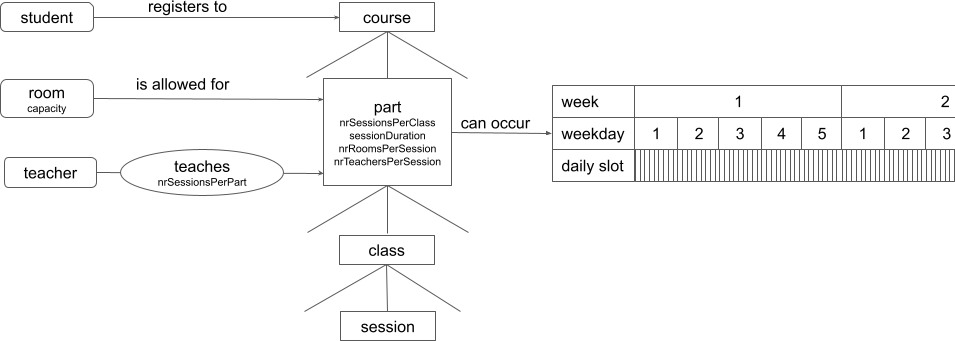
\includegraphics[width=.85\textwidth]{img/utp_entity_model.png}
\caption{Entity model}
\label{fig:utp-entity-model}
\end{figure*}

\subsection{Entity model}
\label{sec:entity-model}
The entity model of a {\UTP} instance defines its schedule horizon, course structure and resources, as well as the properties of entities and the relational maps (see Figure~\ref{fig:utp-entity-model}).  
First, the model uses a time grid that decomposes into weeks, weekdays and daily slots, % (see Figure~\ref{fig:utp-time-grid}),
the number of which is instance-specific.
Weeks share the same weekdays and weekdays the same daily slots.
The latter make up 24 hours and have the same duration (e.g. 24 daily slots will represent 1 hour each, 1440 daily slots represent 1 minute each).
%\marc{C'est pas forcément mesuré en minutes ... Dans nos exemples oui, mais justement c'est custom.
%Il faudrait dire "The latter makes up 24 hours and have the same duration, meaning that 3 dailyslots will represent 8 hours each, or 1440 dailyslots represent 1 minute each." ?}
Note that neither successive weeks nor successive weekdays are assumed to be consecutive.
The schedule horizon is implicitly defined by the series of time slots mapping to week, weekday and daily slot combinations.
Slots hence serve as time points to represent start and end times of course sessions and to measure durations (session length, travel times).

% % For one-column wide figures use
% \begin{figure}[h]
% % \includegraphics{utp-time-grid.eps}
% \caption{{\UTP} 3-layered time grid}
% \label{fig:utp-time-grid}
% \end{figure}

Courses have a tree-structure wherein each course (i.e., course topics) decomposes into parts (lecture, practical work \ldots), parts into classes, and classes into sessions.
Class sessions are the elementary tasks to schedule when solving a {\UTP} instance
and the model fixes their number, duration and sequencing.
On the one hand, the classes of a course part are decomposed into an identical number of sessions of equal duration, both constants being part-specific.
Although this approach forbids alternative class decompositions using variable session durations, 
it %provides flexibility for handling sessions independently wrt. scheduling and resource allocation.
%Fixed decompositions also 
facilitates the formulation of requirements which depend on clear-cut sessions (e.g., planning parallel sessions ``mid-way'' through a course).
On the other hand, the model requires that the sessions of a class be ranked and sequenced accordingly in any solution.
Note that sessions are considered uninterruptible and, in particular, may not overlap two days. 

{\UTP} resources fall into 3 types, namely, rooms, teachers, students (gathered into groups).
All the resources of an instance are declared and typed in the entity model.
In practice, various restrictions resulting from upstream processes apply on the resourcing and timing of courses.
Basic restrictions come in the form of compatibility constraints that list the suitable rooms, eligible teachers, candidate students and allowed times for the different courses 
(e.g., faculties prescribing degree-specific time grids, departments implementing room pooling policies, %alternative 
teachers applying for courses, student registrations). %registering to courses).
Such constraints are built in the entity model but scoped differently depending on resource types.
Specifically, each course part is assigned sets of possible start times, rooms and teachers which propagate automatically to all its sessions.
As for students, course registrations are listed separately and %the possible students for a session are those registered to the course it sits in.
any student registered to a course is considered a possible candidate for each of its sessions.

Beyond plain compatibility, resource utilization is subject to demand and capacity constraints.
Since modalities differ from one environment to the next, the language supports both disjunctive and cumulative resources as well single- and multi-resource sessions. 
Students, teachers or rooms qualify as cumulative resources if they 
can attend, teach or host simultaneous sessions. %, respectively.
Cumulative resources are paramount to meet flexible attendance requirements (e.g., students assigned optional tutoring sessions that may overlap with mandatory courses) or to handle multi-class events (e.g., rooms hosting joint exam or conference sessions).
The schema assumes no limit on the number of parallel sessions teachers and students may attend.
Rooms however may only host class sessions whose cumulated headcount
is within their capacity.
Upper bounds on room capacity and class size are encoded for all rooms and classes in the entity model with the possibility to leave room capacity unbounded (e.g., virtual rooms). 
Note that all resources default to cumulative resources but this assumption may be overridden using disjunctive rules on a per resource basis.
% a {\UTP} instance may freely mix disjunctive and cumulative resources. 

A multi-resource session is a session requiring multiple resources of the same type. %at any point in time.
The need for sessions using multiple rooms or teachers arises in many practical situations (e.g., multi-room sessions for hybrid teaching, joint supervision of practical work sessions, exams requiring several adjudicators).
The number of resources required per session is typically fixed on course parts and  
such restrictions are expressed in the entity model through cardinality constraints. %that are lifted to course parts. 
Specifically, each course part indicates the number of teachers required per session 
and whether its sessions are single- or multi-rooms.
Multi-room sessions impose specific constraints:
allocated rooms are disjunctive for the time of the session only and their total capacity is considered for hosting the students attending the session.
Note that the model allows for sessions without teachers or rooms (e.g., unsupervised student projects). 
%a {\UTP} instance may freely mix single- and multi-resource sessions as well as disjunctive and cumulative resources. 

The entity model also encodes flow constraints that govern the distribution of students and teachers over courses. 
These constraints %relating to the distribution of students and teachers over courses 
are usually elicited ahead of scheduling during registration and capacity planning stages (e.g., departments distributing session volumes among designated teachers). 
As mentioned above, students only register for courses, not for classes nor sessions, and solving a {\UTP} instance involves determining student-to-class assignments that are consistent with the course structure.
Specifically, every student must be assigned a single class in each part of a course he has registered to and must attend all sessions of these classes. 
Group nesting constraints may also be stated between classes %. %to enforce equality or set inclusion relations between their sets of participants.
%These constraints serve 
to implement course-specific or cross-course sectioning policies (e.g., aggregating student groups bottom-up from practicals to lectures, enforcing identical groups between classes of different courses of a curriculum).
As for staff distribution, each teacher is assigned a fixed volume of sessions in each course part he is eligible for, leaving teacher-to-session assignment decisions to solvers.

Note finally that the language provides the ability to label entities and define custom classes of elements (e.g., teams of teachers, blocks of rooms). %that complement the built-in types. 
%Entities sharing the same label form a type of their own named after the label.
Labels complement built-in types and entity identifiers as a means to select entities within rules.
  


%Rules may then help to enforce instance-specific scheduling or resource allocation constraints on any entity or group of entities, e.g. casting a problem instance as a pure disjunctive scheduling problem.

%First, teachers are explicitly represented on par with rooms. Student groups may optionally be modelled too to cater for workflows where student sectioning is performed ahead of session scheduling. 

%The {\UTP} schema also differs on the way sessions are time-framed in a class. Indeed a class' sessions are just chronologically ranked and specific scheduling requirements are enforced per class (e.g., periodicity) or across classes (e.g., simultaneity) through explicit rules.
%while leaving the opportunity to jointly state and solve both problems. Second, it represents teachers explicitly, allows for class sessions requiring multiple resources (e.g., multi-room or -teacher sessions),
%and supports resource distribution constraints (e.g., eligible teachers and their workload per course part measured in sessions).
%and rooms %(including virtual rooms) 


We formalize below the entity model and introduce notations that will be used thereafter.
Let ${\ENTITY}$ denote the set of entities
and ${\SESSION}$ the set of sessions.
${\ENTITY}$ is partitioned into   
a set of courses ${\COURSE}$, 
a set of course parts ${\PART}$, 
a set of classes ${\CLASS}$, 
a set of students ${\STUDENT}$, 
a set of teachers ${\TEACHER}$,
a set of rooms ${\ROOM}$,
and the singleton domain of courses ${\COURSES}$ 
(${\COURSES}=\myset{\COURSE}$). 
Let 
%${\COURSES}$ denote the course domain, 
%${\COURSE}$ the set of courses (${\COURSES}=\myset{\COURSE}$), 
%${\PART}$ the set of course parts, 
%${\CLASS}$ the set of classes, 
%${\SESSION}$ the set of sessions, 
%${\STUDENT}$ the set of students, 
%${\TEACHER}$ the set of teachers, 
%and 
%${\ROOM}$ the set of rooms.
$
{\TYPE}
=
\myset{
{\COURSES}, 
{\COURSE},
{\PART},
{\CLASS},
{\STUDENT},
{\TEACHER},
{\ROOM}
}
$
denote the set of entity types
(${\ENTITY}=\setunion{X}{\TYPE}{X}$)
and 
$
{\prec}
=
\myset{
({\COURSES},{\COURSE}),
({\COURSE},{\PART}),
({\PART},{\CLASS}),
({\CLASS},{\SESSION}),
({\STUDENT},{\COURSE}),
({\TEACHER},{\PART}),
({\ROOM},{\PART})
}
$
denote the relation over 
${\TYPE}\cup\myset{\SESSION}$ 
that models the course hierarchy
and the distribution of resource types over course components.
${\prec^{*}}$
%${\preceq^{*}}$
denotes the transitive %and reflexive 
closure of
${\prec}$ 
over
${\TYPE}\cup\myset{\SESSION}$
and
${\maptype{X}{Y}}:X\rightarrow2^{Y}$
denotes the function mapping each element of $X$ to its set of compatible elements in $Y$
for each pair %$(X,Y)$ such that 
%$X{\preceq^{*}}Y$.
$X{\prec^{*}}Y$.
For instance, 
${\maptype{\STUDENT}{\COURSE}}$ 
represents the distribution of students over courses, 
${\maptype{\COURSE}{\PART}}$ 
the decomposition of courses into course parts,
and ${\maptype{\STUDENT}{\PART}}$ 
the inferred distribution of students over course parts.
The functions corresponding to the pairs of $\prec$
are directly encoded in the entity model
and the remaining functions are defined inductively using recursive aggregation. 
Rule (\ref{model:hierarchy}) below models the hierarchical decomposition of course elements\footnote{$\sqcup$ denotes the disjoint union operation, i.e. set union over pairwise disjoint sets.}
and
Rule (\ref{model:transitivity}) is the closure rule over 
%$\preceq^{*}$. 
$\prec^{*}$. 
%Rule (\ref{model:symmetry}) enforces symmetry over all compatible pairs,
%and Rule (\ref{model:selfmap}) completes the model with self-maps. 

%\todo[inline]{i en indice dans les équations suivantes, formulation non expliquée. $d_i$ serait l'ensemble des couples (a,b) de la relation tels que a=i ?}
%\vincent{Dans ce cas, comme d est une fonction, ça serait plutôt $d^{Y,Z}(i)$}
%\marc{On en discutait avec DG et effectivement c'est ce qu'on a conclu. Cependant, plus tard cette notation est réutilisée avec en indice des ensembles de valeurs. Il faut donc faire attention à bien introduire cette notation.
%De plus je rajouterais une petite remarque : $\forall (X,Y)$ et non $\forall X,Y$ ?}

\begin{multline}
\forall (X,Y) \in  \myset{ ({\COURSES},{\COURSE}), ({\COURSE},{\PART}), ({\PART},{\CLASS}), ({\CLASS},{\SESSION}) }: \\
Y=\setpartition{i}{X}{\map{X}{Y}{i}} \label{model:hierarchy}
\end{multline}
\begin{multline}
\forall X,Y,Z \in {\TYPE}\cup\myset{\SESSION}:\\
\mbox{\hspace{-10em}}X\preceq^{*} Y\preceq^{*} Z 
\Rightarrow \\
(\forall i \in X:
\map{X}{Z}{i}=\setpartition{j}{\map{X}{Y}{i}}{\map{Y}{Z}{j}}
 \label{model:transitivity})
%%
%%\forall X,Y \in {\TYPE}:
%%X\preceq^{*} Y 
%%\Rightarrow 
%%(\forall i \in X, j \in Y:
%%j \in \domarg{X}{Y}{i} \Leftrightarrow i \in \domarg{Y}{X}{j}
%%) \label{model:symmetry}\\
%%
%\forall X \in {\TYPE}\cup\myset{\SESSION},
%i \in X:
%\domarg{X}{X}{i} = \myset{i} \label{model:selfmap}
%%
\end{multline}

%We shall denote by
%${\RANK}$
%the range of session ranks,
%${\maptype{\RANK}{\SESSION}}:\RANK\rightarrow2{^\SESSION}$
%the rank-based partitioning of sessions,
%and
%${\LABEL}$
%the set of labels 
%(${\LABEL}\subseteq2^{{\ENTITY}}$)
%completed 
%with the whole set of entities %to mock label optionality
%($\ENTITY\in{\LABEL}$)
%and singleton entities %to support identity-based selection
%($\myset{\myset{e}\ |\ e\in{\ENTITY}}\subseteq{\LABEL}$).
%As discussed in section~\ref{sec:rules},
%labels are optional filters used in rules to select entities
%hence the formal inclusion of $\ENTITY$ in ${\LABEL}$ to mock label optionality.
%Likewise, entity identifiers are used as an alternative to labels
%hence the inclusion of singleton entities in ${\LABEL}$.

%------------------------------------------------------------
%------------------------------------------------------------
\subsection{Predicates and constraints}
\label{sec:constraints}
{\UTP} constraints apply to pairs, called e-maps, which associate an entity with a non-empty subset of its compatible sessions.
%which we call e-maps. 
Constraints are built with predicates whose signature includes e-map variables%ranging over the set of e-maps
, the number of which is referred to as the arity of the predicate. 
Note that some predicates may also accept parameters.
Let 
${\EMAP}=
\setunion{X}{\TYPE}
\myset{(e,S')\ |\ e\in X,S'\subseteq\map{X}{\SESSION}{e}\wedge S'\neq\emptyset}$
denote the set of e-maps,
a {\UTP} constraint has the form
\begin{align}
c((e_1,S_1),\ldots,(e_m,S_m),p_1,\ldots,p_n) \label{rule:constraint}
\end{align}
where 
$c$ is a predicate symbol of arity $m$,
$(e_1,S_1)$, $\ldots$, $(e_m,S_m)$ are e-maps ($(e_i,S_i)\in{\EMAP}$, $i=1\ldots m$) 
and 
$p_1,\ldots,p_n$ are values for the parameters of $c$ ($n\geq0$).


Every predicate may be used indistinctly with e-maps defined on course elements or on resources.
E-maps defined on resources are interpreted as conditional session-to-resource assignments
when checking constraints 
whereas e-maps defined on course elements are unconditional assignments since they model constitutive sessions.
In other words, 
a constraint is only evaluated
on the sessions whose assignments in the considered solution are consistent with its e-map arguments.\footnote{Formally, let $\var{E}{\SESSION}{e}$ be the variable denoting the set of sessions assigned to entity $e$ and $S'_1,\ldots,S'_m$ be sets of sessions, the conditionality of a constraint $c$ is stated as follows: 
$(\var{E}{\SESSION}{e_1}=S'_1 \wedge \var{E}{\SESSION}{e_m}=S'_m)
\Rightarrow
(c((e_1,S_1),\ldots,(e_m,S_m),p_1,\ldots,p_n)
\Leftrightarrow
c((e_1,S_1\cap S'_1),\ldots,(e_m,S_m\cap S'_m),p_1,\ldots,p_n))$.
}
It follows that 
a constraint is evaluated on every session that is mapped to a course element.
In particular, constraints that apply exclusively to course elements are unconditional. 
Note also that the use of e-maps that model the whole set of sessions compatible with an entity 
will necessarily constrain any session that may be assigned to this entity.


%Every predicate may be used indistinctly with e-maps defined on course elements or on resources which we call c-maps and r-maps, respectively. R-maps are interpreted conditionally since they map a resource to some of its possible sessions whereas c-maps model unconditional assignments since they model constitutive sessions of course elements. In other words, a constraint must be evaluated on every session of every c-map in its scope but only on the sessions of its r-maps whose resource assignment is compatible with the proposed solution.\footnote{Formally, let $\var{E}{\SESSION}{e}$ be the variable denoting the set of sessions assigned to entity $e$ and $S'_1,\ldots,S'_m$ be sets of sessions, the conditionality of a constraint $c$ is stated as follows:  $(\var{E}{\SESSION}{e_1}=S'_1 \wedge \var{E}{\SESSION}{e_m}=S'_m) \Rightarrow (c((e_1,S_1),\ldots,(e_m,S_m),p_1,\ldots,p_n) \Leftrightarrow c((e_1,S_1\cap S'_1),\ldots,(e_m,S_m\cap S'_m),p_1,\ldots,p_n))$.}
%effectively assigns to the resource of the r-map.
%(see Rule (\ref{rule:conditionality})).
%It follows that constraints applying exclusively to c-maps are unconditional. Besides, the scoping of e-maps that model the whole set of sessions compatible with an entity will constrain every session assigned to a resource or constitutive of a course element.
%%The rule below %(\ref{rule:conditionality}) models the conditionality of constraints.

%{\footnotesize{
%\begin{multline}
%\forall S'_1,\ldots,S'_m\in{\SESSION}:
%(\var{E}{\SESSION}{e_1}=S'_1 \wedge \var{E}{\SESSION}{e_m}=S'_m)
%\Rightarrow\\
%(c((e_1,S_1),\ldots,(e_m,S_m),p_1,\ldots,p_n)
%\Leftrightarrow
%c((e_1,S_1\cap S'_1),\ldots,(e_m,S_m\cap S'_m),p_1,\ldots,p_n))
%\label{rule:conditionality}
%\end{multline}
%}}

\begin{table*}[!ht]
\resizebox{\textwidth}{!}{%
\centering
\begin{tabular}{|l|l|l|l|}
\hline
\textbf{Name}               & \textbf{Arity} & \textbf{Parametric} & \textbf{Semantics}\\ \hline

%assign\_slot               & 1         & yes   & Assign a slot or slot tuple to a session\\ \hline
%assign\_room               & 1         & yes   & Assign a set of room to session in entry\\ \hline

%allocation\_group           & 1        & no    & Domain allocation for class with group in the solution\\ \hline
%part\_schedule              & 1        & no    & Allowed start time slots for sessions\\ \hline
%domain\_class\_group        & 1        & no    & Allowed groups for classes (solution input)\\ \hline
%domain\_session\_teacher    & 1        & no    & Allowed teachers for sessions\\ \hline
%domain\_class\_room         & 1        & no    & Allowed rooms for sessions\\ \hline

{\SAMEDAILYSLOT}            & 1         & no    & Sessions start on the same daily slot\\ \hline
{\SAMEWEEKDAY}              & 1         & no    & Sessions start on the same weekday\\ \hline
{\SAMEWEEKLYSLOT}           & 1         & no    & Sessions start on the same weekly slot\\ \hline
{\SAMEWEEK}                 & 1         & no    & Sessions start the same week\\ \hline
{\SAMEDAY}                  & 1         & no    & Sessions start the same day\\ \hline
{\SAMESLOT}                 & 1         & no    & Sessions start at the same time\\ \hline
{\FORBIDDENPERIOD}          & 1         & yes   & Sessions cannot start in the time period\\ \hline
{\ATMOSTDAILY}              & 1         & yes   & The number of sessions scheduled in the daily period is upper-bounded\\ \hline
{\ATMOSTWEEKLY}             & 1         & yes   & The number of sessions scheduled in the weekly period is upper-bounded\\ \hline
%implicit\_sequenced\_sessions & 1 & \multicolumn{4}{|c|}{no} & All sessions in classes are sequenced\\ \hline
{\SEQUENCED}                & $\geq2$   & no    & Sessions are sequenced\\ \hline
{\WEEKLY}                   & 1         & no    & Sessions are weekly \\ \hline

{\NOOVERLAP}                & 1         & no    & Sessions cannot overlap\\ \hline
{\TRAVEL}                   & 1         & yes   & Travel time is factored in if sessions hosted in the rooms\\ \hline

{\SAMEROOMS}                & 1         & no    & Sessions are hosted in the same room(s)\\ \hline
{\SAMESTUDENTS}             & 1         & no    & Sessions are attended by the same student(s)\\ \hline
{\SAMETEACHERS}             & 1         & no    & Sessions are taught by the same teacher(s)\\ \hline

{\ADJACENTROOMS}            & 1         & yes   & Sessions are hosted in the adjacent rooms\\ \hline

{\TEACHERDISTRIBUTION}      & $\geq2$   & yes   & Distributes teacher workload over classes\\ \hline

\end{tabular}
}
\caption{Catalog of {\UTP} predicates}
\label{tab:predicate_catalog}
\end{table*}


% 
% \newcolumntype{M}[1]{>{\raggedright}m{#1}}
%\begin{table}[!h]
%    \centering
%    \begin{tabular}{|l|M{2cm}|*{7}{c|}}
%        \hline
%        \multirow{2}{4em}{Name} & \multirow{2}{4em}{Entity} & \multirow{2}{1cm}{Arity} & \multicolumn{4}{|c|}{Parameter} & \multirow{2}{6em}{Conditional} & \multirow{2}{10em}{Explication}   \\
%        \cline{4-7}
%           & & &name& type& number& type & &    \\
%        \hline
%
%
%assign\_slot & All & max 1 & slot & max 1 & min 1 & slots  & yes & Assign a slot or slot tuple to a session\\ \hline
%
%allocation\_group&Part& max 1  & \multicolumn{4}{|c|}{no}  & no  & Domain allocation for class with group in the solution\\ \hline
%
%assign\_room  & Course, Part, Class, Sessions, Teacher, Student &max 1 &rooms &  1 & min 1 &room & yes & Assign a set of room to session in entry\\ \hline
%
%\multirow{2}{6.5em}{at\_most\_daily} & \multirow{2}{2cm}{Course, Part, Class, Teacher, Room, Student }& \multirow{2}{4em}{max 1} &count & 1 & 1 & slot &\multirow{2}{4em}{ yes} &\multirow{2}{4em}{ Limit a number of session in intervalle } \\ 
%\cline{4-7}
%  & & &first& 1& 1& slot & &    \\
%  \cline{4-7}
%  & & &last& 1& 1& slot & &    \\
%\hline
%at\_most\_weekly & Course, Part, Class, Teacher, Room, Student & max 1 & count &  1 & 1 & slot & yes & Limit a number of session in intervalle \\ \hline
%
%connected\_room &  Course, Part, Class, Teacher, Room, Student & max 1 & roomChain & min 1  & min 2 & room [ordered]  & yes & Session need connected rooms \\ \hline
%
%disjunctive\_group & Student & max 1 & \multicolumn{4}{|c|}{no} & yes & A group cant have overlap of 2 sessions  \\ \hline
%
%disjunctive\_room & Room   & max 1 & \multicolumn{4}{|c|}{no} & yes & A room cant host 2 sessions at same moment  \\ \hline
%
%disjunctive\_teacher & Teacher & max 1 & \multicolumn{4}{|c|}{no} & yes & A teacher cant gives  classes at same moment\\ \hline
%
%domain\_class\_group & Class & max 1 & \multicolumn{4}{|c|}{no} & no & A subset of group to classes (need solution)\\ \hline
%
%domain\_session\_teacher & Session & max 1 & \multicolumn{4}{|c|}{no} & no & A subset of teacher for sessions\\ \hline
%
%domain\_class\_room &Class & max 1 & \multicolumn{4}{|c|}{no} & no & A subset of room for class \\ \hline
%
%\multirow{2}{5.5em}{forbidden\_slot} & \multirow{2}{4em}{All} & \multirow{2}{4em}{max 1} & first & 1 & 1& slot & \multirow{2}{4em}{yes} & \multirow{2}{4em}{A session cant take slot in intervalle} \\
%  \cline{4-7}
%  & & &last& 1& 1& slot & &    \\
%\hline
%
%implicite\_sequenced\_sessions & Class & max 1 & \multicolumn{4}{|c|}{no} & no & All sessions in classes are sequenced\\ \hline
%
%\multirow{2}{9em}{not\_consecutive\_rooms} &\multirow{2}{2cm}{ Course, Part, Class, Teacher, Student} &\multirow{2}{4em}{ max 1} & minGap & 1 & 1 & slot & \multirow{2}{4em}{yes} & \multirow{2}{4em}{If 2 sessions have rooms in tuple then need a gap of mingap to walk from one the other} \\ 
%  \cline{4-7}
%  & & &rooms& 2 & min 1 & room,label & &   \\
%\hline
%
%part\_schedule & all & max 1 & \multicolumn{4}{|c|}{no}  & yes & we allowed time part value\\ \hline
%
%same\_daily\_slot & all & min 1 & \multicolumn{4}{|c|}{no} & yes & all slots of  selected sessions  are equal to the same daily slot \\ \hline
%
%same\_day  & all & min 1 & \multicolumn{4}{|c|}{no} & yes & all slots of  selected sessions  are equal to the same day \\ \hline
%
%same\_rooms & Course, Part, Class, Session, Teacher, Student  & min 1 & \multicolumn{4}{|c|}{no} & yes & all set rooms of  selected sessions  are equal \\ \hline
%
%same\_slots & all  & min 1 & \multicolumn{4}{|c|}{no} & yes & all slots of  selected sessions  are equal \\ \hline
%
%same\_teachers & Course, Part, Class, Session, Room, Student  & min 1 & \multicolumn{4}{|c|}{no} & yes & all set teachers of  selected sessions  are equal \\ \hline
%
%same\_week & all & min 1& \multicolumn{4}{|c|}{no} & yes & all slots of  selected sessions  are equal to the same week \\ \hline
%
%same\_weeklyday & all & min 1 & \multicolumn{4}{|c|}{no} & yes & all slots of  selected sessions  are equal to the same weekly day \\ \hline
%
%same\_weeklyslot & all & min 1 & \multicolumn{4}{|c|}{no} & yes & all slots of  selected sessions  are equal to the same weekly slot \\ \hline
%
%sequenced & Course, Part, Class, Session & min 1 & \multicolumn{4}{|c|}{no} & no & Sessions are ordered in the horizon slot (i.e i < j slot[session[i]] < slot[session[j]] \\ \hline
%
%teacher\_repartition & Class & min 2& class & min 2 & 1 & option  & no & repartition of teacher into a differentes classes of part \\ \hline
%
%weekly & Course, Part, Class, Session & min 1& \multicolumn{4}{|c|}{no} & no & A session tuple is weekly \\ \hline
%    \end{tabular}
%    \caption{Catalog of {\UTP} predicates}
%    \label{tab:catalog_constraint}
%\end{table}

Table \ref{tab:predicate_catalog} lists the predicates of the language
and indicates which are variadic or parametric.
The first predicates 
\texttt{\SAMEDAILYSLOT},
\ldots,
%\texttt{\SAMEWEEKDAY},
%\texttt{\SAMEWEEKLYSLOT},
%\texttt{\SAMEWEEK},
%\texttt{\SAMEDAY} and
\texttt{\SAMESLOT}
enforce common restrictions on the start times of the targeted sessions (e.g., sessions starting the same day).
Additionally,
any start time interval may be forbidden 
by passing its start and end points 
as parameters to 
predicate \texttt{\FORBIDDENPERIOD}.
Predicates \texttt{\ATMOSTDAILY}
and
\texttt{\ATMOSTWEEKLY}
upper-bound
the number of sessions
scheduled daily or weekly
within the given time interval.
\texttt{\SEQUENCED}
is a n-ary predicate ($n\geq2$)
which constrains
the latest session of the $i$-th e-map 
to end before
the earliest session of $i+1$-th e-map ($i=1..n-1$).
Predicate 
\texttt{\WEEKLY}
ensures sessions
are scheduled %weekly
on the same weekly slot
without presuming any particular sequencing.
Predicate
\texttt{\NOOVERLAP}
ensures sessions do not overlap in time
and is typically used to model disjunctive resources.
Predicate \texttt{\TRAVEL}
factors in any travel time
incurred between consecutive sessions
hosted in distant rooms.
The travel time matrix is a parameter of the predicate.
\texttt{\SAMEROOMS},
\texttt{\SAMESTUDENTS}
and
\texttt{\SAMETEACHERS}
require that sessions be assigned to the same set of rooms,
students or teachers.
Predicate 
\texttt{\ADJACENTROOMS}
require that sessions be hosted in 
adjacent rooms 
based on an adjacency graph passed as a parameter.
Lastly, 
predicate \texttt{\TEACHERDISTRIBUTION}
distributes the volumes of sessions represented by the different e-map arguments 
among different teachers. Teachers and session volumes are parameters of the predicate.
%\marc{Je pense qu'un exemple ici pourrait être intéressant ?
%"Two teachers may share a class where one does the first half of the sessions and the other one the last half."}

%\marc{Je remonterai le tableau pour qu'il apparaisse plus tôt ?}

%------------------------------------------------------------
%------------------------------------------------------------
\subsection{Rules}
\label{sec:rules}
%For instance, unconditional start time restrictions using predicates such as {\SAMEDAILYSLOT} or {\FORBIDDENPERIOD}  may be enforced on any set of sessions bound to a course, a part, a class or more generally to the course domain. Conversely, start time restrictions on a set of sessions bound to a resource will only be enforced on those which are eventually assigned to the resource.
%Predicates serve to constrain the possible sessions of resources (e.g., unavailabilities of a teacher) or the constitutive sessions of course elements (e.g., periodicity of a class). 
%e-maps may then be adjusted to constrain candidate sessions of resources (e.g., teacher unavailability), constitutive sessions of course elements (e.g., class periodicity), or individual sessions (e.g., session sequencing and parallelization).
Rules are used to state conjunctions of constraints and in particular single constraints. %and in particular individual (singleton) constraints.
Each rule is defined by a universally quantified formula which restricts the domains of the e-map variables of a given predicate.
The collection of constraints hence represented is obtained by instantiating the predicate with each tuple of e-maps belonging to the cross-product of the domains.
E-map domains are not given in extension
but represented using a language of selectors
which provides a comprehension syntax to generate and filter e-maps.
Let 
${\SELECTOR}$
denote the language of e-map domain selectors,
%(${\SELECTOR}\subseteq({\TYPE}\times{\LABEL}\times{2^{\RANK}})^{n}$).
a {\UTP} rule has the form %is a tuple 
\begin{align}
c(F_1,\ldots,F_m,p_1,\ldots,p_n)
\end{align}
and is interpreted by %The semantics of a rule $(c,D_1,\ldots,D_m,p_1,\ldots,p_n)$ is 
the %quantified 
formula
\begin{multline}
\forall (e_1,S_1)\in\denote{F_1},\ldots,(e_m,S_m)\in\denote{F_{m}}:\\
c((e_1,S_1),\ldots,(e_m,S_m),p_1,\ldots,p_n)
\label{rule:rule}
\end{multline}
where 
$c$ is a predicate symbol of arity $m$,
$F_1,\ldots,F_m$ are selectors ($F_i\in{\SELECTOR}$, $i=1\ldots m$),
$p_1,\ldots p_n$ are values for the parameters of $c$ ($n\geq0$),
and
$\denote{F_i}$
denotes the domain of e-maps represented by
selector 
$
F_i\in{\SELECTOR}
$
.

The language of selectors allows 
to target entities based on type, label or identity
and
to filter their sets of sessions
based on session rank and mutual compatibility with other entities.
It is complete in the sense 
that it allows to construct any domain of e-maps whose entities share the same type.
For instance, one may construct the e-maps which
associate any of the rooms labeled \texttt{Building-A}
with the compatible sessions of rank 2 or 4 
that are also constitutive of course \texttt{course-1} or class \texttt{class-3}.
A selector
combines a generator and an optional list of filters.
Generators and filters are triples 
$
(T_i,L_i,O_i)
$
consisting of
an entity type
$
T_i%\in{\TYPE}
$,
an entity label or identifier
$
L_i%\in{\LABEL}
$
and
a subset of session ranks
$
O_i%\subseteq{\RANK}
$ (a.k.a., session mask),
the latter two elements being optional.
A selector 
matches any e-map
whose entity satisfies the type, label and identifier constraints of the generator
and whose %set of sessions 
image includes any compatible session
satisfying the mask of the generator
and one of the filters.
Note that rules featuring empty selectors are discarded during the flattening stage. 
%Selectors are encoded as attributes in the {\XML} language
%using a syntax that borrows from the CSS selector language.
%For instance, the above example would be encoded by the following XML fragment: 
%\todo[inline]{Marc : Rajouter une phrase pour décrire brièvement la figure 3}

\begin{figure*}[h]
\centering
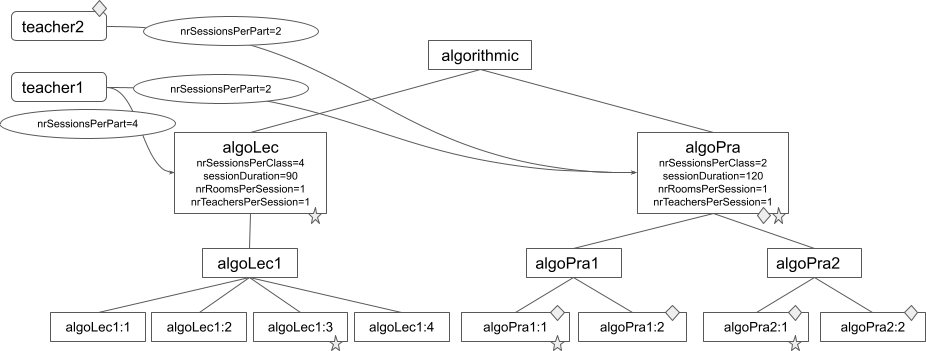
\includegraphics[scale=0.5]{img/utp_rule_1.png}
\caption{Rule interpretation}
\label{fig:utp-rule-1}
\end{figure*}

%\marc{Mettre ici le dernier paragraphe sur la sélection des rangs ? Et l'exemple en fin de section ?}
Let
${\RANK}$
denote the range of session ranks,
${\maptype{\RANK}{\SESSION}}:\RANK\rightarrow2{^\SESSION}$
the rank-based partitioning of sessions,
and
${\LABEL}$
the set of labels 
(${\LABEL}\subseteq2^{{\ENTITY}}$)
completed 
with the whole set of entities to mock label optionality
($\ENTITY\in{\LABEL}$)
and singleton entities to support identity-based selection
($\myset{\myset{e}\ |\ e\in{\ENTITY}}\subseteq{\LABEL}$),
the language of selectors
is the set 
$
\cup_{n\geq1}({\TYPE}\times{\LABEL}\times{2^{\RANK}})^{n}
$.
%where each 
Each selector 
$
d=((T_1,L_1,O_1),\ldots,(T_k,L_k,O_k))
$
%($k\geq1$)
decomposes into a generator
$
(T_1,L_1,O_1)
$
and a possibly empty list of filters
$
((T_2,L_2,O_2),\ldots,(T_k,L_k,O_k))
$.
%A session $s$ is said to satisfy triple
%$
%(T_i,L_i,O_i)
%%\in({\TYPE}\times{\LABEL}\times{2^{\RANK}})
%$
%if
%it is compatible with
%an entity of type $T_i$ and label $L_i$ 
%($s\in\map{T_i}{\SESSION}{L_i}$)\footnote{
%%Let $X\subseteq Y$,
%$
%{\map{Y}{\SESSION}{X}}
%$
%denotes
%$
%\setunion{i}{X\cap Y}{\map{Y}{\SESSION}{i}}
%$.
%}
%and 
%if it satisfies mask $O_i$, i.e., its rank is included in $O_i$
%($s\in\map{\RANK}{\SESSION}{O_i}$).
%A selector 
%$
%d=((T_1,L_1,O_1),\ldots,(T_k,L_k,O_k))
%$
$d$ matches any e-map
whose entity has type $T_1$ and label $L_1$ and whose image includes any compatible session satisfying mask $O_1$ and any of the filters.
The set of e-maps
$\denote{d}$
matched by $d$
%selector 
%$
%d%=
%%((T_1,L_1,O_1),\ldots,(T_k,L_k,O_k))
%$
%represents
%the set of e-maps 
is defined by
\begin{multline*}
\denote{d}=
\bigcup\limits_{e\in{T_1}}
%\myset\left\{(e,S')
\Big \{(e,S')
\ |\ 
%e\in T_1\cap L_1,
S'=
\mape{T_1}{\SESSION}{\myset{e}\cap L_1}
%\cap 
%\map{\RANK}{\SESSION}{O_1}
\;\cap \\
\bigcup\limits_{i=2\ldots k}
{
\mape{T_i}{\SESSION}{L_i}
\cap
\mape{\RANK}{\SESSION}{O_1\cap O_i}
\wedge
S'\neq\emptyset
}
\Big \}
\end{multline*}

where
$
{\mape{X}{Y}{X'}}
=
%$
%denotes
%$
\bigcup\limits_{i\in X'}{\map{X}{Y}{i}}
$
with
$X'\subseteq X$
.

Figure~\ref{fig:utp-rule-1} is a toy example to illustrate the interpretation of rules.
The course \texttt{algorithmic} has 2 parts : lecture part \texttt{algoLec} and practice part \texttt{algoPra}.
There is 1 lecture class, taught by \texttt{teacher1}, and 2 practical classes taught by \texttt{teacher1} and \texttt{teacher2}.
%\todo[inline]{Marc : harmoniser notations}
The lecture class has 4 sessions and each practical class has 2 sessions.
Figure~\ref{fig:utp-rule-1} illustrates the flattening of the following rules: 
%on a simple model consisting of 2 teachers and & course subdivided into 2 parts, 3 classes and 8 sessions. The first rule forbids a time period for 

{\footnotesize{
\begin{multline}
\texttt{\mbox{\hspace*{-1em}}{\FORBIDDENPERIOD}((<(\TEACHER,{teacher2},\_)>,9120,9240)}\label{rule-example-1}\\
\end{multline}
\begin{multline}
\texttt{\mbox{\hspace*{-1em}}{\SEQUENCED}(<(\CLASS,\_,\myset{3}),(\PART,{algoLec},\_)>,}\\
\texttt{<(\CLASS,\_,\myset{1}),(\PART,{algoPra},\_)>)\label{rule-example-2}}
\end{multline}
}}

Rule~\ref{rule-example-1}
requires that \texttt{teacher2} has no session between 8am and 10am the second day of week 2.
In this example, the time grid has 1440 slots a day and 5 days a week, meaning that slot %value\footnote{Each possible session slot is mapped to a single value. All possible values make up the domain of a session.} 
9120 (resp. 9240) corresponds to 8am (resp. 10am) the second day of week 2.
The selector includes no mask and no filter hence matches with all possible sessions of \texttt{teacher2} 
as indicated with diamonds on Figure~\ref{fig:utp-rule-1}. 
The resulting domain of e-maps is the singleton $\myset{(teacher2,\map{\TEACHER}{\SESSION}{teacher2})}$
and the rule is flattened into a single \texttt{\FORBIDDENPERIOD} constraint. %$\myset{\map{\TEACHER}{\SESSION}{teacher2}}$.
Rule~\ref{rule-example-2}
%requires that the first practical session in Algorithmic \todo[inline]{Marc : pourquoi algo ?} start after the third lecture.
requires that the first sessions of the practices start after the third session of the lecture.
The two selectors include a filter. The first selector matches with all class sessions of rank 3 in part \texttt{algoLec}, 
and the second matches with all class sessions of rank 1 in part \texttt{algoPra} as indicated with stars on the figure.
The rule is flattened into 2 \texttt{\SEQUENCED} constraints corresponding to the cross product of the e-map domains $\myset{(algoLec1,\map{\RANK}{\SESSION}{3}\cap\map{\PART}{\SESSION}{algoLec})}$
and $\myset{(algoPra1,\map{\RANK}{\SESSION}{1}\cap\map{\PART}{\SESSION}{algoPra}),(algoPra2,\map{\RANK}{\SESSION}{1}\cap\map{\PART}{\SESSION}{algoPra})}$.

%------------------------------------------------------------
%------------------------------------------------------------
\subsection{Solution}
\label{sec:solution}
The solution component includes assignment decisions
relating to the choice of slots and resources for sessions,
the placement of students in groups and
the assignment of groups to classes.
The solution hence represented may be partial, even empty 
and does not have to be consistent with the built-in constraints or the rules of the instance.
The support for partial solutions allows to tackle subproblems using separate {\UTP} instances and solution seeds.
For instance, a scheduling instance may be defined on the basis of partial and consistent solutions pre-generated for the student sectioning and resource allocation subproblems.
Likewise, the support for inconsistent solutions is paramount to repair solutions that have become inconsistent due to unforeseen changes.

%As mentioned before, 
Student groups are considered a by-product of student sectioning.
For this reason, groups may only be listed in the solution component, not in the entity model, and defined both by the students they include and the classes they are assigned to. 
This sectioning process is subject to different constraints. 
First, students are partitioned into groups and students are inextricably bound to their group.
Second, groups may only include students with identical course registrations.
Third, group-to-class assignments must comply with any subgroup inclusion constraint stated in the entity model.

%Let ${\SLOT}$ denote the range of slots defining the schedule horizon, $\maptype{\PART}{\SLOT}$ denotes the set of allowed slots defined for each course part in the entity model. 
%$\maptype{\SESSION}{\SLOT}$ shall denote the set of slots assigned to each session in a solution component.
%Let ${\GROUP}$ denote the set of groups defined in a solution, $\maptype{\GROUP}{\STUDENT}$ and $\maptype{\CLASS}{\GROUP}$ shall denote respectively the students making up each group and the groups making up each class.



% %The schema thus allows to cast university timetabling problems either as cumulative or disjunctive scheduling problems that subsume student sectioning or not.


% \paragraph{Paragraph headings} Use paragraph headings as needed.
% \begin{equation}
% a^2+b^2=c^2
% \end{equation}

% For one-column wide figures use
%\begin{figure}
% Use the relevant command to insert your figure file.
% For example, with the graphicx package use
%  \includegraphics{example.eps}
% figure caption is below the figure
%\caption{Please write your figure caption here}
%\label{fig:1}       % Give a unique label
%\end{figure}
%
% For two-column wide figures use
%\begin{figure*}
% Use the relevant command to insert your figure file.
% For example, with the graphicx package use
%  \includegraphics[width=0.75\textwidth]{example.eps}
% figure caption is below the figure
%\caption{Please write your figure caption here}
%\label{fig:2}       % Give a unique label
%\end{figure*}
%
% For tables use
%\begin{table}
% table caption is above the table
%\caption{Please write your table caption here}
%\label{tab:1}       % Give a unique label
% For LaTeX tables use
%\begin{tabular}{lll}
%\hline\noalign{\smallskip}
%first & second & third  \\
%\noalign{\smallskip}\hline\noalign{\smallskip}
%number & number & number \\
%number & number & number \\
%\noalign{\smallskip}\hline
%\end{tabular}
%\end{table}





%------------------------------------------------------------
%------------------------------------------------------------
\section{Related work}
\label{sec:related-work}

We highlight here the main differences between the {\UTP} language and the {\ITC} schema ({\ITC} for short) \cite{2018muller,ITC2019}.

%the two approaches use the same temporal representation but {\ITC} leaves the possibility to configure the granularity of daily slots in each instance (${\DAILYSLOT\in\myset{1\ldots 1440}}$)  while it is set to the minute in {\UTP}. Nevertheless, any granularity may be used in {\UTP} by filtering the series of allowed slots in course parts and by re-scaling session duration and travel time data.
A first difference between the two frameworks lies in the representation of the possible times a class can meet.
In {\UTP}, a class is defined by a single sequence of sessions of equal duration and the problem is to schedule each session.
In {\ITC}, a class is given alternative fixed session schedules ({\texttt{times}} elements in the {\XML} schema) and the problem is to choose one of the schedules for the class.
A schedule is the repetition over a set of weeks of one or more sessions that have the same duration and start on specific days of the week at the same predefined time (daily slot).
The two representations are not reducible to one another.
For instance, alternative schedules using different session durations cannot be modeled in {\UTP}.
Conversely, class schedules where sessions do not necessarily start on the same daily slot cannot be modeled in {\ITC}.
Nevertheless, basic class schedules may be represented in either approach by stating {\ITC} constraints or {\UTP} rules on classes.
For instance, a class meeting every week on the same day and the same daily slot, both being subject to time restrictions, may be modeled using \texttt{\SAMEDAILYSLOT}, \texttt{\WEEKLY} and \texttt{\FORBIDDENPERIOD} constraints.
The implementation of a more comprehensive reduction method %for alternative schedules 
%(based, for instance, on a dedicated {\UTP} predicate) 
will be the subject of future work.

%Another difference lies in the representation of resources and the constraints governing their distribution and allocation.
%On the one hand, 
Second, 
{\ITC} represents alternative course configurations
by introducing an intermediate layer in the course hierarchy 
that sits between courses and parts.
The configurations of a course typically differ in their number of (sub)parts
and are mutually exclusive from a student sectioning standpoint, that is, 
a registered student must be assigned a single configuration and attend all of its parts.
This feature is not currently supported in {\UTP}.
As for resources, {\UTP} explicitly represents teachers on par with rooms %and allows to specify their workload in each course part %(i.e., the number of sessions to teach)
whereas {\ITC} only models rooms.
{\UTP} also provides the flexibility to allocate different resources within a class 
(and specify teacher workload in particular) %(i.e., the number of sessions to teach)
whereas the same room must be allocated in {\ITC}.
Additionally, {\UTP} supports multi-resource sessions whereas {\ITC} is restricted to single-room sessions.

The two constraint languages also present important differences.
While {\ITC} constraint predicates apply to classes,
{\UTP} predicates apply to any set(s) of sessions
and may be used in particular on individual sessions, hence granting finer-grained control.
Besides, {\UTP} rules and the selector language allows to constrain any class of resources or course elements in a concise way.

Lastly, the {\ITC} schema addresses the timetabling problem as a combinatorial optimization problem.
It includes a cost function weighting 4 criteria which respectively penalize the choice of sessions and rooms for the classes, the violations of constraints and the overlapping of sessions per student.
In its current version, the {\UTP} language addresses the problem as a hard constraint satisfaction problem.
The integration of soft constraints and the possibility of aggregating penalties or preferences, either in solution generation or repair contexts, is under investigation.

%Student groups 
% near-identical course structure: no course configuration element
% no time elements in UTP classes. Alternative class times are fixed in ITC
% OK time elements in extension -> unusitable for loosely constrained class programs
% OK impossible to express k weekly slots with different starting slots. In UTP: use sameWeeklySlot with masks.
% OK impossible to enforce different constraints bettwen first period of a course (amorcage) and the rest => ok for us with masks
% KO: times with different #sessions and session length. 
% => solution per session (vs per class) : slot + romms + teachers


%Sectioning:: as itc (parent class)
%Ressources
%- rooms: travel in ITC => using constraint travel in UTP.
%- new: teachers.
%- students: no change.
%- OK groups. Admin and computational needs.
%- Domain constraints
%- by default, all resources are cumultative (explain). Avec contrainte (disjunctive):: no overlap on romms/etc. 
%- allowed slot (applies to all sessions of a part's classes) : ITC via time elements. Adequate for "grid systems". 
%- allowed rooms and allowed teachers (worklaod per part = prescribed number of sessions)
%- single or multi-room/teacher session in UTP.
%- possibly different resources between sessions of a class (unless addiiotnal rules:: sameRoom, sameTeacher, ...)
%Rules language
%- ITC: class-level constraints vs session-level constraints on UTP
%- Labelling: simplifies constraint expression to look up entities
%Solution
%seul ajout: group-to-class and student-to-group
%Résolution: UTP == SAT vs Opt/gestion prefs => pas de priorites, pondérations, etc
%

\section{{\UTP} implementation}
\label{sec:model_implementation}

%%%
% fusion XML
% outil XML > JSON
% PoC : MZN
% Expérimentations
%%%

%The \UTP{} language is a domain-specific language to model a class of university timetabling problems.
%We decided to solve the instances using constraint programming (\CP{}).
In this section, we present the toolchain illustrated in Figure~\ref{fig:toolchain} that is used to process and convert \UTP{} instances to \CP{} compatible formats. We then briefly introduce a generic \CP{} model and its alternative implementation in \MINIZINC{} \cite{MZN} and \CHR{} \cite{Fruhwirth_TechReport_92,Fruhwirth_CP_94,Fruhwirth_JLP_98,Fruhwirth_CHR_09,Fruhwirth_Abdennadher_CHR_03,Fruhwirth_Raiser_2011}. Lastly, we present the experiments carried out on a real instance.

\begin{figure}
    \centering
    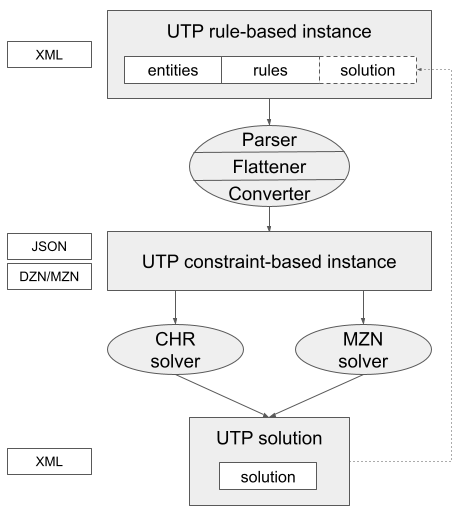
\includegraphics[width=\columnwidth]{2022_APIA/img/utp_toolchain.png}
    \caption{The \UTP{} toolchain}
    \label{fig:toolchain}
\end{figure}

% intro
%The \UTP{} language is easy to describe a timetabling problem instance, but it has to be converted into constraints to be solved.
%We developed a tool that translate a \UTP{} instance into a \CP{} instance.
%We implemented two solvers: one using \MINIZINC{} and one using constraint logic programming with \CHR{}.
%Both solvers were used to solve a real instance.

\subsection{Merger, Parser, Flattener and Converter}
The \UTP{} language is embedded in \XML{}
and comes with a \PHP{} tool 
which combines a parser, a rules flattener and a converter.
The flattener processes rules to generate collections of {\UTP} constraints
and the converter transforms the resulting constraint-based instance into 
\CP{} solver compatible formats based on \JSON{} and \DZN{} (\MINIZINC{} instance format).
%format which may be read by .

The tool also allows to merge \UTP{} instances
into one.
%A \UTP{} instance may thus be built by merging smaller instances
This is useful as data and requirements are usually captured separately for different curriculae or even courses. % and by different stakeholders (e.g., faculty departments, course owners, teachers, etc.).
For instance, one would typically merge all curriculum instances in a faculty. %of individual courses.
% \XML{} files.
%
%The tool was developed in \PHP{} and is available on our website \cite{USPsite}.
%\todo[inline]{Je ne comprends pas la transition (ou l'absence de transition) avec la section suivante. On est d'accord que le "traducteur" XML -> CP-JSON applique ce qui est décrit en 4.2 non ? Dans ce cas, ça manque d'une phrase de liaison (ou alors ce dernier paragraphe devrait être coupé en 2, et mis en partie en 4.2. }
Two \UTP{} instances can be merged as long as they share the same time grid.
All resources (rooms, teachers and students) with the same identifier are merged, e.g. a student may appear in original files and will be present once in the merged files with all its subscribed courses and assigned groups.
Two files with a course sharing the same identifier cannot be merged.
The rule merging raises the question of the labels and the scope of a rule.
Here there are two solutions: either the labels are merged as is, and if two files share the same labels then the rules using the label will apply to all the resources of the merged file with the label ; either the labels are modified to be unique.
%
The current version of the tool does not change labels, thus the user must be careful with the use of labels in files.

% Présenter le modèle PPC
\subsection{\CP{} Model and Solvers}

The \CP{} model of a \UTP{} instance includes instance data, decision variables, built-in constraints of the entity model and constraints generated from the rules set. %using the {\UTP} predicates.
The input data are a transcription of the entity model and include the time grid, the course hierarchy, the set of resources and the various properties of entities and their relations.
The decision variables model the groups chosen for a class and the group, slot, rooms and teachers chosen for each session.

Sectioning constraints partition students into groups based on course registrations, %, i.e., students may not be placed in the same group if they register to different courses.
forbid group sharing between classes of a course part and impose that every student (through its group) attends each part of a course he is registered to.
They also implement the parent relationships between classes and make sure the maximum size of a class is never exceeded by the total headcount of its groups. 

Resource distribution constraints define the domains of resource allocation variables (i.e. allowed rooms and teachers for each session)
and enforce cardinality restrictions regarding the number of teachers needed for each session, the number of sessions taught by each teacher in a course part, whether a room is mandatory in a part, and whether a session is single-room or multi-rooms.

Scheduling constraints define the domains of session scheduling variables (i.e. allowed slots per session),
and ensure sessions do not span over two days and are sequenced based on their rank in each class.
Default cumulative capacity constraints apply to all resources to guarantee each room has sufficient capacity to host its assigned sessions at any one time.
Dedicated constraints handle the particular case of multi-room sessions to make sure 
each room is disjunctive while it is being used,
groups are freely distributed and split over the rooms,
and the cumulated capacity of the rooms is considered for hosting.

Lastly, each {\UTP} predicate has a custom constraint-based implementation to achieve the desired semantics.



As a proof of concept, we implemented a {\CP} model for the class of {\UTP} problems using \MINIZINC{} and running {\GECODE} \cite{GECODE} as a back-end solver.
This model makes use of global constraints, notably constraint \texttt{cumulative} \cite{beldiceanu2002new} which serves to handle both cumulative and disjunctive resources.
We implemented a second solver using constraint logic programming in \CHR\ (Constraint Handling Rules) in order to take advantage of the propagation of constraints on variable domains as in \CP\ but also of the global structure of the problem (\CHR\ allows to manipulate symbolic expressions and not only domains).
We used \CHRPP\ \cite{barichard_stephan_2019} to implement the model and solve the instances.



\subsection{Experiments}
We carried out experiments on a real-life instance modeling the second semester of the last year of Bachelor in Computer Sciences at Université d'Angers (available at \cite{USPsite}).

The instance consists of 5 mandatory courses and 2 optional courses to choose amongst 4, 24 course parts and 42 classes, 67 students pre-divided into 4 groups, 12 teachers and 8 rooms.
The time grid is decomposed into 12 weeks, 5 weekdays and 1440 daily slots.
Note that courses last 80 minutes in this Faculty and must be placed on a specific time grid ranging from 08\string:00am to 07\string:50pm with session starting every 90 minutes to account for breaks.
The instance includes 46 rules, namely, 13 constraints \texttt{\WEEKLY}, 16 \texttt{\SEQUENCED}, 2 \texttt{\SAMESLOT}, 5 \texttt{\SAMEWEEK}, 5 \texttt{\SAMEROOMS} and 5 \texttt{\SAMETEACHERS}.

Both \MINIZINC{} and \CHRPP{} solvers were run with an Intel Core i7-10875H 2.30GHz and solved the instance in less than 5 seconds.
%
Source codes for the \MINIZINC{} and \CHRPP{} models are available on our website \cite{USPsite}.
%------------------------------------------------------------
%------------------------------------------------------------
\section{Conclusion and perspectives}
\label{sec:conclusion}
We introduced in this paper a domain-specific language for university course timetabling. 
The language allows to model a wide variety of curriculum-based timetabling problems
such as those encountered in French universities. 
%This is particularly the case in French universities where students are divided into groups that attend all the courses they are registered for.
It provides support for typical timetabling entities (students, sessions, teachers, rooms, etc.) and features (student sectioning, resource distribution, session scheduling, resource allocation) and includes a rules language to easily express constraints (sequencing, periodicity, etc.).
Rules allow to target any subset of domain entities and sessions and enforce timetabling-specific predicates.

We used the language to encode a real instance (Bachelor courses of a French university) and 
implemented a tool chain to convert the \XML\ instance files into solver-compatible formats.
In order to validate our approach, we implemented a \CSP\ model capable of solving \UTP\ instances. 
We implemented this \CSP\ model in \MINIZINC\ and \CHR\ and produced solutions for the considered instance.

%We believe that the \UTP\ language is the first link in a chain of processes whose purpose is to create a timetable that can evolve according to the random events occurring during the period on which it is built.

%We are currently working on improving the second link, which consists of building the timetable from scratch. 

We are currently working on different extensions of the language and the back-end solvers.
First, we intend to represent preferences and priorities in order to support timetable optimization and repair tasks.
Second, the current {\CP} models may be improved using dedicated scheduling constraints, search strategies and heuristics and take advantage of model simplication and reformulation techniques.
Another objective is to improve scalability by testing our solvers on large-scale instances aggregating different curriculae or converted from academic benchmarks.
Lastly, we intend to investigate the revision of timetables to manage unexpected events (e.g.  unavailability of a teacher, late registration of students) or to support incremental solution construction. 

%The \UTP\ language makes it possible to model a problem ex nihilo, but also makes it possible to amend an existing model by adding constraints when an event occurs (e.g. unexpected unavailability of a teacher, late registration of students). 
%Even if the \UTP\ language allows to express these random events, the \CSP\ and \CHR models must take them in order to calculate new solutions. Moreover, they must do so in an incremental and dynamic way in order to respond to the succession of events that may occur over the period of application of the schedule. 
%It is after having dealt with this last link that the resolution methods will make it possible to solve the problem of designing and updating a timetable as it occurs in everyday life.


%\davidl{CP dur : pas d'optimisation. En parler en intro / conclusion ? -> extension du catalogue de prédicat et de l'aspect optimisation plus tard}


%\subsection{Travaux antérieurs}
%
%Les en-têtes sont également en 12 points gras.
%
%Il n'y a pas nécessairement d'espacement entre les paragraphes.
%
%Les références à la Bibliographie peuvent être de la forme
% \cite{key:foo} o\`u \cite{foo:baz}.  Les numéros correspondent à
% l'ordre d'apparition dans la bibliographie, pas dans le texte.
% L'ordre alphabétique est conseillé.
%
%\subsubsection{Les autres éléments}
%
%Vous pouvez également utiliser des sous-sous-sections (comme c'est le cas ici). Taille 10 points, gras.
%
%Pour les figures, elles doivent être insérées à l'aide de l'environnement \verb|figure| et avoir une légende numérotée.
%
%L'inclusion d'images peut se faire à l'aide de la commande
%\verb|\includegraphics|.
%
%Vous pouvez utiliser des listes d'éléments sans changer l'item (ici le tiret) :
%\begin{itemize}
%  \item item1
%  \item item2
%  \item ...
%\end{itemize}
%
%Vous pouvez utiliser aussi l'environnement \verb|\paragraph|.
%
%\paragraph{Ce ceci est un paragraphe.} Remarquez que le titre du paragraphe se termine par un point, et qu'il n'est PAS numéroté.
%
%Essayez si possible de ne pas utiliser de subdivision supplémentaire dans votre article car il risquerait de perdre en lisibilité. 
%\section{Pagination}
%
%Afin que l'éditeur puisse assembler vos contributions en un seul volume, veillez impérativement à :
%\begin{itemize}
%  \item ne PAS ajouter de numéros de page ;
%  \item ne PAS changer les marges (ou tout autre élément de mise en page) ;
%  \item d'une manière générale, ne PAS modifier le style fourni ou ne PAS lui ajouter des éléments de formatage qui changent le visuel, sinon votre contribution risque de ne pas être formatée de la même manière que celle des autres.
%\end{itemize}
%
%En principe, les articles doivent faire au plus 8 pages.
%
%\section{Biblio}
%
%Dans la section suivante, vous voyez deux exemples de références. Si vous utilisez bib\TeX, alors spécifiez l'utilisation du style plain à l'aide de la commande habituelle : \verb|\bibliographystyle{plain}|.
%
\section*{Acknowledgments}
%Ce travail est partiellement financé par le projet Thélème octroyé aux universités d'Angers et du Mans dans le cadre du PIA3.
This work is partially funded by project Thélème granted to the universities of Angers and Le Mans under PIA3 program.
%Les remerciements s'expriment juste avant la bibliographie, à l'aide d'une Section non numérotée.
%
%
%\begin{thebibliography}{9}
%\bibitem{foo:baz}
%U. Nexpert,
%{\em Le livre,}
%Son Editeur, 1929.
%\bibitem{key:foo}
%I. Troiseu-Pami,
% Un article intéressant,
%{\em Journal de Spirou}, Vol. 17, pp. 1-100, 1987.
%\end{thebibliography}


\bibliographystyle{plain}
\bibliography{ref_APIA}

\end{document}

